\section{Metodología de pruebas} 
Como metodología de pruebas para el proceso haremos uso 
de \href{https://owasp.org/www-pdf-archive/OWASP_Application_Security_Verification_Standard_4.0-en.pdf}{OWASP Application Security Verification Standard (ASVS) 4.0} 
que proporciona una base para probar los controles técnicos de seguridad de las aplicaciones web. El proyecto clasifica
 los distintos controles en tres niveles. En este caso cubriremos todos los controles incluidos en el \textbf{nivel 2}.\\

 Para abordar el proceso de pentesting los dividiremos en las fase definidas en el 
 apartado 2.1.2, para la ejecución del proceso de pentesting ejecutaremos todas las fases menos la 
 de explotación y Postexplotación.\\

 Fases de del proceso de pentesting aplicadas:\\
 \begin{itemize}
     \item Alcance y términos de la prueba de intrusión.
     \item Recolección de información.
     \item Análisis de vulnerabilidades.
     \item Generación de informes.
 \end{itemize}
 
 Detallaremos el proceso en las siguientes secciones.

\newpage

\subsection{Alcance y términos de la prueba de intrusión}
Para cubrir este punto se genera un documento de plan de pruebas para cada sistema objetivo, este documento es 
importante para fijar el objetivo sobre el que se ejecutará la prueba de penetración, 
los tipos de ataque que se ejecutaran, herramientas y la metodología que se utilizaran, así como los documentos que se entregaran 
como resultado de la ejecución del proceso de pentesting.\\

Normalmente este documento se suele entregar al dueño del sistema objetivo de la prueba de penetración para que 
lo valide y de su aceptación antes de iniciar el proceso de pentesting.\\

También, en muchos casos es necesario, sobre todo en sistemas de producción, restricciones horarias a la hora de ejecutar el proceso.\\

Este documento, en caso de legar a fases de explotación y postexplotación, debe ser ampliado para detallar en que consistirán el 
proceso de explotación y postexplotación y los posibles efectos que pueden acarear al sistema de pruebas.\\

Para los sistemas de prueba elegidos se han creado dichos los documentos en la siguiente 
\href{https://github.com/M0l1n3ta/PFG/tree/master/Reportes/PPR%20-%20Plan%20de%20pruebas}{ruta} \cite{web3}\\

\subsection{Recolección de información}

Para este punto de proceso se suelen utilizar numerosas herramientas y depende mucho de la persona que ejecute 
el proceso de pentesting.\\ 

Pero siempre es de utilidad partir de un análisis estático de código ya que el resultado de dicho 
análisis ayuda enormemente al pentester de distintas formas:

\begin{itemize}
    \item Las vulnerabilidades encontradas en dicho proceso pueden ser utilizadas para utilizar las herramientas más 
    oportunas para cada error detectado, así como crear las pruebas necesarias para reproducir los ataques necesarios 
    para explotar dicho error.
    \item Las vulnerabilidades encontradas en este proceso son añadidas como base para el análisis dinámico.
    \item Suele acortar los tiempos del proceso de recolección de información.
\end{itemize}

Como resultado del análisis estático de código se genera un reporte donde, a parte de enumerar los errores
encontrados y las distintas métricas de calidad del código, se añade un apartado dedicado a detallar las 
vulnerabilidades encontradas, así como las medidas que deben ser tenidas en cuenta para mitigar o resolver el defecto encontrado.\\

\newpage
Este reporte puede ser presentado ante el dueño del sistema de prueba y el equipo de desarrollo para abordar mejor 
el proceso de solución de los defectos encontrados, así como mejoras en la calidad del código más allá de los defectos de seguridad.\\

Además, se suele instruir al equipo de desarrollo para que hagan uso de una de las ventajas que tiene SonarQube 
que es la integración con los entornos de desarrollo a través de SonarLint. Esto permite a los desarrolladores 
estar al tanto de los defectos que presenta el software directamente en el entorno de desarrollo y solventar 
los defectos antes de que se realice el análisis estático de código de las versiones entregadas. El del complemento SonarLint
 ha permitido en multitud de proyecto la detección temprana de defectos y su solución, así como la mejora 
 de las distintas métricas de calidad del código.\\

La generación de dicho reporte se ha automatizado en un pequeño programa que detallamos en el siguiente apartado.


\subsection{Generación reporte análisis estático de código}

Para generar los reportes de análisis estático de código nos ayudaremos de una pequeña utilidad creada en Python, que hemos 
denominado \textbf{“SonarQube Reporting Tool”}, implementada en Python que hace uso de los servicios web disponibles en SonarQube
para recopilar los datos de los escáneres realizados e integrarlos con una plantilla base del 
reporte para generar un reporte final con los datos extraídos por la herramienta más los comentarios del pentester.

La aplicación esta disponible en GitHub, la podemos descargar en instalar con los siguientes comandos:
\begin{verbatim}
    git clone https://github.com/M0l1n3ta/SonarQubeReportingTool.git
    cd SonarQubeReportingTool
    pip3 install -r requirements.txt
\end{verbatim}

Para ejecutar la aplicación:
\begin{verbatim}
    python3 static_analysis_report_generator.py
\end{verbatim}

\newpage
Para generar el reporte seleccionamos la primera opción \textbf{“Reporting tool”}:
\begin{figure}[!htb] 
    \centering
    \captionsetup{width=1\linewidth}   
    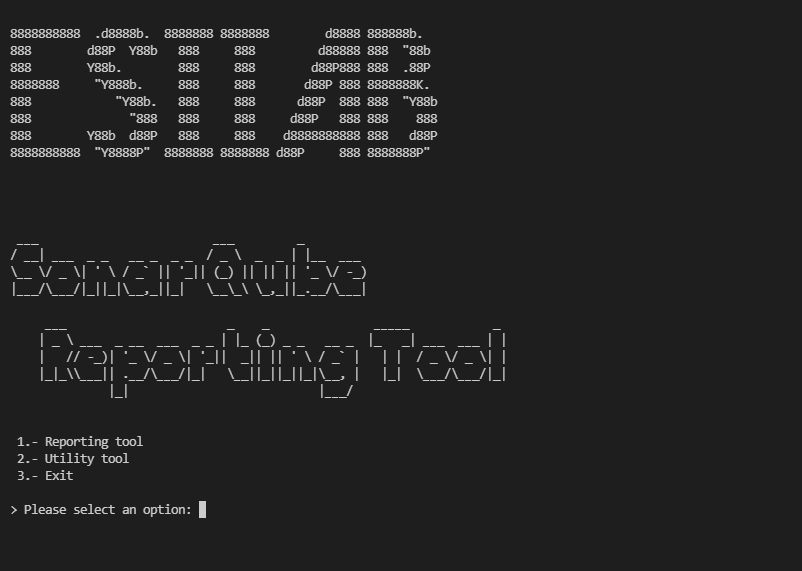
\includegraphics[scale=0.8]{./imagenes/017_SonarQubeReportTool_1.png}
    \caption{SonarQube Reporting Tool.}  
    \label{fig:15 - SonarQube Reporting tool}
\end{figure}

Seleccionamos el Proyecto de SonarQube del cual queremos generar el reporte estático de código:
\begin{figure}[!htb] 
    \centering
    \captionsetup{width=1\linewidth}   
    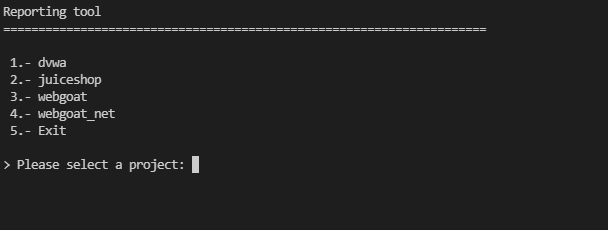
\includegraphics[width=\linewidth]{./imagenes/017_SonarQubeReportTool_2.png}
    \caption{Seleccionar proyecto Sonarqube.}  
    \label{fig:16}
\end{figure}

\newpage
Finalmente seleccionamos la segunda opción \textbf{“Generate detailed report”} para generar el reporte:

\begin{figure}[!htb]
    \centering
    \captionsetup{width=1\linewidth}     
    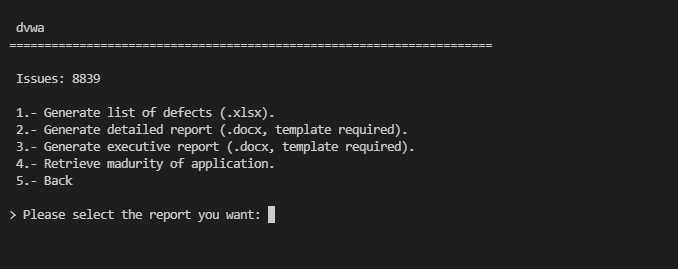
\includegraphics[scale=0.8]{./imagenes/017_SonarQubeReportTool_3.png}
    \caption{Generar reporte análisis estático}  
    \label{fig:17}
\end{figure}

El reporte se generará en el directorio de ejecución:

\begin{figure}[!htb] 
    \centering
    \captionsetup{width=1\linewidth}     
    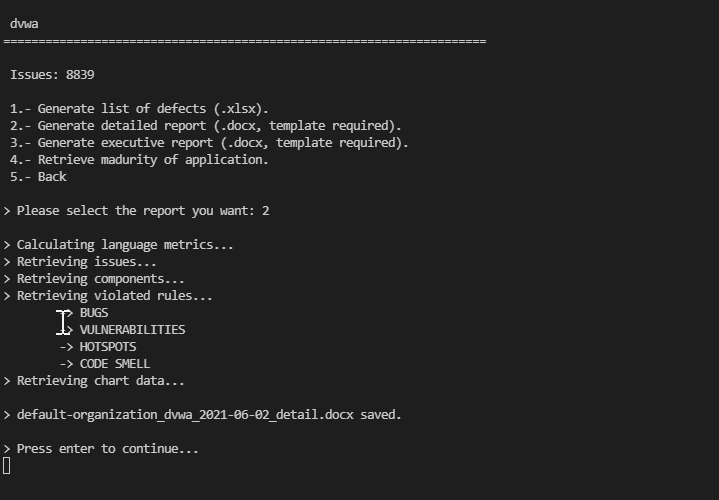
\includegraphics[width=\linewidth]{./imagenes/017_SonarQubeReportTool_4.png}
    \caption{Resultado generación reporte análisis estático}  
    \label{fig:18}
\end{figure}

\newpage
\subsection{Análisis de vulnerabilidades.}
Con la información de recogida en la fase anterior más y la que pueda añadir el pentester se crea un plan de pruebas 
para su ejecución configurando las peticiones para que pasen a través del proxy de OWASP ZAP.

\begin{figure}[!htb]
    \centering
    \captionsetup{width=1\linewidth}  
    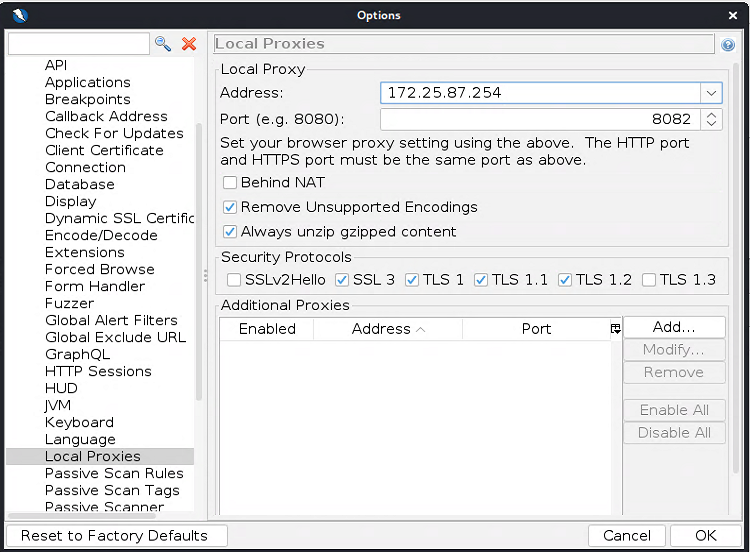
\includegraphics[scale=0.9]{./imagenes/031_OWASPZAP_LocalProxy.png}
    \caption{Configuración}  
    \label{fig:localProxyOWASPZap}
\end{figure}

Con todas las peticiones generadas por el plan de pruebas más las que el pentester decida añadir se irán almacenado 
en una sesión de OWASP ZAP.\\

Una vez finalizado el plan de pruebas lanzamos el spider para que descubra nuevas rutas en la aplicación

\begin{figure}[!htb]
    \centering
    \captionsetup{width=1\linewidth}  
    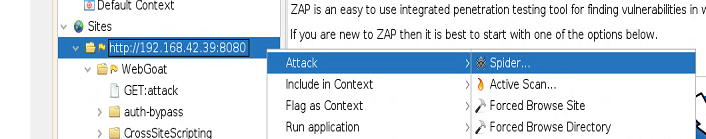
\includegraphics[width=\linewidth]{./imagenes/03_01_WebGoat_ZapProxySpider.png}
    \caption{OWASP ZAP Spider}  
    \label{fig:OWASPZap Spider}
\end{figure}

\newpage
Con la url añadidas desde el plan de pruebas, más la detectadas con el proceso de \textbf{“Spider”}, más la que el 
pentester considere añadir lanzamos el proceso de análisis dinámico de código. Para ello seleccionamos la url de pruebas 
y con el segundo botón seleccionamos \textbf{“Attack > Active Scan”}

\begin{figure}[!htb]
    \centering
    \captionsetup{width=1\linewidth}  
    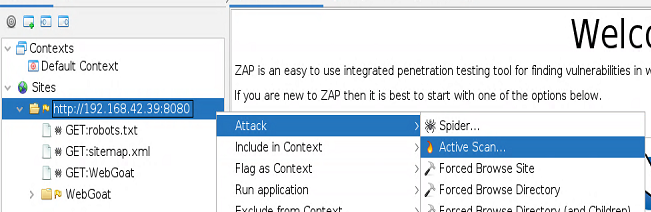
\includegraphics[width=\linewidth]{./imagenes/03_02_WebGoat_ZapProxyActiveScan.png}
    \caption{OWASP ZAP Active Scan}  
    \label{fig:OWASPZap Active Scan}
\end{figure}

Para iniciar el escáner dinámico seleccionamos la política \textbf{“Default Policy”} e iniciamos con 
\textbf{“Start Scan”}, como se muestra en la figura /ref{fig:OWASPZap Active Scan Start}:

\begin{figure}[!htb]
    \centering
    \captionsetup{width=1\linewidth}   
    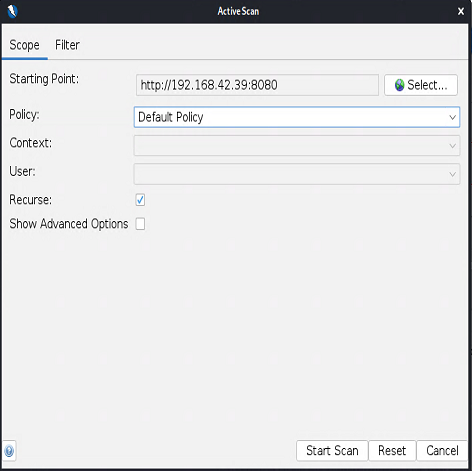
\includegraphics[scale=0.9]{./imagenes/03_03_WebGoat_ZapProxyActiveScanStart.png}
    \caption{OWASP ZAP Active Scan Start}  
    \label{fig:OWASPZap Active Scan Start}
\end{figure}

\newpage
Una vez finalizado escáner dinámico se revisan las alertas para descartar los que se consideren falsos positivos y 
se genera el reporte de análisis dinámico. Para generar el reporte de análisis dinámico 
se selecciona en menú la opción \textbf{“Report”}. en nuestro caso generaremos el tipo de Reporte \textbf{HTML} 
como se muestra en la figura \ref{fig:OWASPZapReport}: 

\begin{figure}[!htb]
    \centering
    \captionsetup{width=1\linewidth}   
    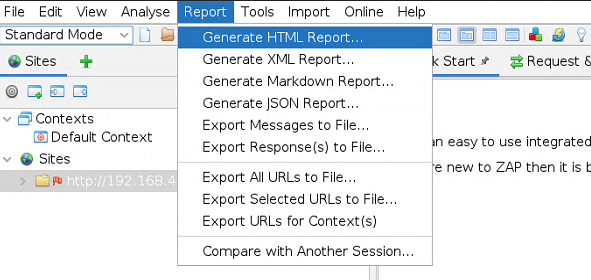
\includegraphics[scale=0.7]{./imagenes/03_04_OWASP_ZAP_Report.png}
    \caption{Reporte OWASP ZAP}  
    \label{fig:OWASPZapReport}
\end{figure}

Y seleccionamos uno de los tipos de reporte:

\begin{itemize}
    \item HML
    \item XML
    \item Markdown
    \item JSON
\end{itemize}

En nuestro caso seleccionaremos el tipo de reporte HTML. Una vez generado el reporte de análisis dinámico es recomendable 
abrir todos los defectos encontrados en un gestor de defectos, tanto los defectos encontrados en el
análisis estático de código como en el  dinámico, e informar al equipo de desarrollo de los mismo y si fuese necesario 
planificar una reunión para abordar la solución a los defectos encontrados.\\

Trascurrido un tiempo se suele generar un reporte de resultado del análisis de seguridad de la versión del software analizada o antes 
del análisis de una nueva versión del software donde se detallará el estado de los defectos encontrados en ese momento. 
\newpage

\subsection{Generación de informes.}
\label{section:GeneracionInformes}

Como resultado el proceso de ejecución de las pruebas de seguridad generaremos los siguientes documentos:

\begin{itemize}
    \item Definición del plan de pruebas de seguridad.
    \item Reporte análisis estático de código.
    \item Plan pruebas para el análisis dinámico.
    \item Reporte análisis dinámico.
    \item Informe resultado ejecución pruebas de seguridad.
\end{itemize}

\newpage